\subsection{Overall Performance}
\label{subsec:overall-performance}

Table~\ref{tab:main-results} presents performance across all agents on 1,017 test scenarios evaluated with three LLMs. React-ADDIE achieves the highest mean score (86.49), demonstrating that integrating the ADDIE framework with ReAct-style reasoning yields superior ISD quality.

React-ADDIE consistently achieves the highest scores across all three LLMs, with particularly strong performance on Gemini-3-Flash (87.61) and GPT-5-mini (88.43). The phase-wise analysis reveals that React-ADDIE leads in Analysis (84.2), Design (84.8), Implementation (84.0), and Evaluation (83.0), while Dick-Carey-Agent excels specifically in Development (84.2) due to its systematic materials creation approach.

A notable observation is EduPlanner's performance degradation on GPT-5-mini (61.43) and Solar-Pro3 (61.46), with particularly weak Development phase scores (48.5). This suggests that EduPlanner's multi-agent architecture may be sensitive to model-specific characteristics, while our theory-based agents show more consistent cross-model performance.

React-ADDIE's integration of ADDIE theory with ReAct-style reasoning outperforms both pure theory-based agents (ADDIE-Agent: 82.96, which uses the same ADDIE framework but with fine-grained 14-tool decomposition) and technique-only approaches (Baseline: 84.07). This suggests that the optimal approach lies in combining established ISD theories with modern agent architectures.

\subsection{Multi-Judge Evaluation}
\label{subsec:multi-judge}

To address LLM-as-a-Judge bias concerns, we employ two judge models from different providers: GPT-4o-mini (OpenAI) and Gemini-2.5-flash-lite (Google). Table~\ref{tab:reliability} summarizes inter-judge agreement and bias metrics.

\begin{table}[t]
\centering
\small
\caption{Inter-judge reliability and bias analysis across 5,183 evaluations.}
\label{tab:reliability}
\begin{tabular}{llc}
\toprule
\textbf{Category} & \textbf{Metric} & \textbf{Value} \\
\midrule
\multirow{3}{*}{Agreement} & Mean Reliability & 0.905 \\
& Std. Deviation & 0.084 \\
& Min / Max & 0.293 / 1.000 \\
\midrule
\multirow{4}{*}{Distribution} & Excellent ($\geq$0.9) & 63.3\% \\
& Good (0.75--0.9) & 31.4\% \\
& Moderate (0.5--0.75) & 5.1\% \\
& Low ($<$0.5) & 0.3\% \\
\midrule
\multirow{2}{*}{Bias} & Gemini-2.5-flash-lite & +0.060 \\
& GPT-4o-mini & -0.060 \\
\bottomrule
\end{tabular}
\end{table}

The high inter-judge reliability (0.905) with 94.7\% of evaluations achieving good or excellent agreement validates our multi-judge protocol. Both judges show minimal systematic bias ($\pm$0.06 points from median), confirming balanced evaluation without provider preference.

%% Figure 4-6 (moved here for earlier placement)
\begin{figure*}[!t]
\centering
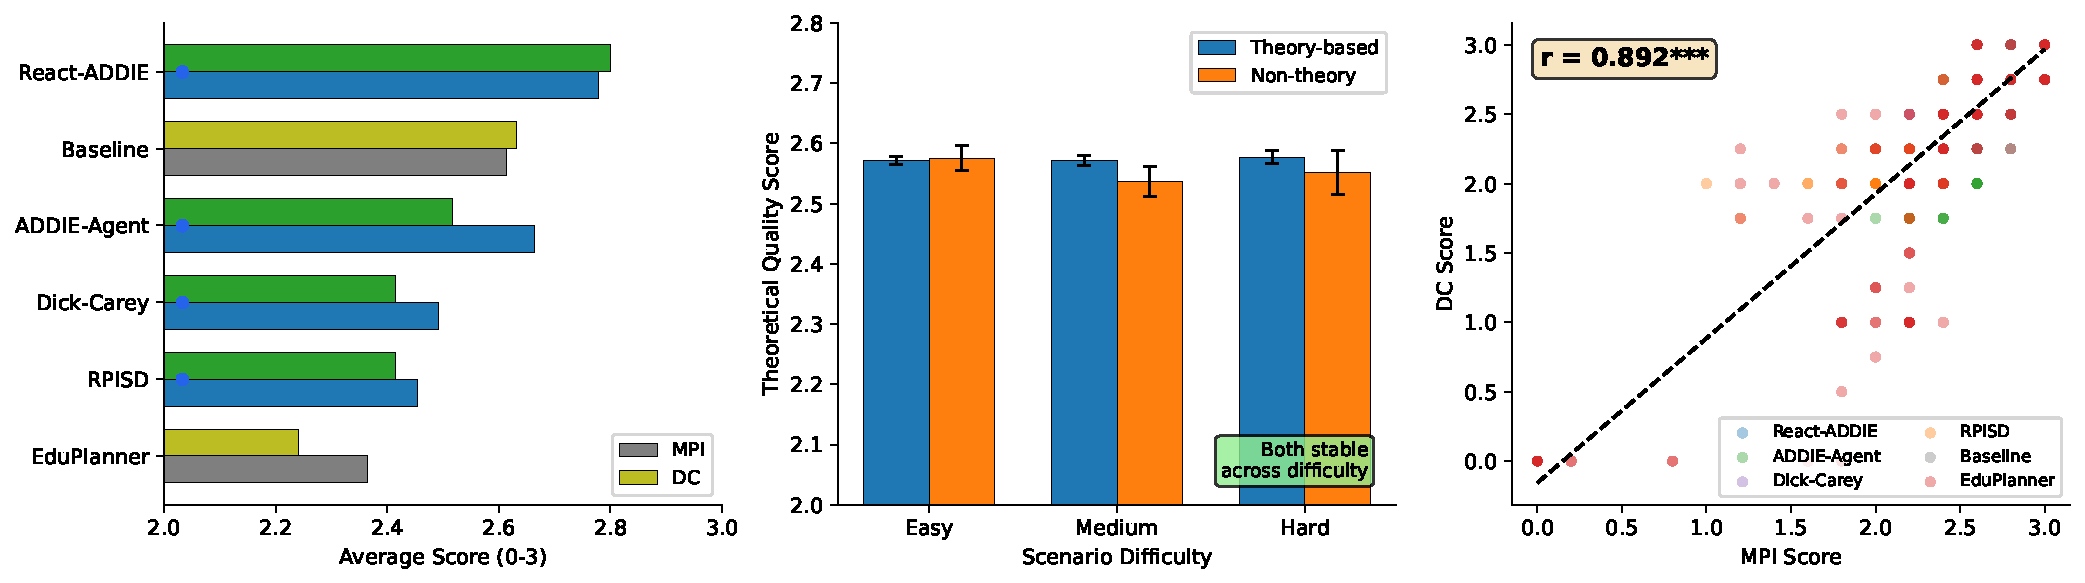
\includegraphics[width=\textwidth]{fig_paper_findings_4_6.pdf}
\caption{Agent comparison and framework validation. \textit{Left panel} presents agent-wise MPI and DC scores with theory-based agents marked, where React-ADDIE leads both dimensions. \textit{Middle panel} shows theoretical quality by difficulty level, demonstrating both agent types maintain stable performance. \textit{Right panel} illustrates MPI-DC correlation ($r = 0.892$), confirming the frameworks capture related but complementary quality aspects.}
\label{fig:findings-4-6}
\end{figure*}

